% !Mode:: "TeX:UTF-8"
\documentclass[a4paper]{nuist}

\begin{document}

\cover{南京信息工程大学本科生毕业论文\LaTeX 模板 \\Version $1.(e^{i\pi}+1)$}{路人甲}{20101301888}{大气科学学院}{大气科学}{路人乙~教授}{二O一六~年~五~月~ 二~日}%此处存在一个bug:pdf不能复制,去掉封面项后可复制尚不知问题所在。
\pagenumbering{roman}
\mytableofcontents

\maketitleofchinese{南京信息工程大学本科生毕业论文\LaTeX 模板V1.0\footnote{本模板制作时间:2014年5月}}{路人甲\footnote{作者:Bruce Y.P. Lee\\通讯地址:\url{yupenglee119@gmail.com}}、人造人\footnote{第二版修改者LiR\\E-mail:\url{stuliren@outlook.com}}}{大气科学}

\pagenumbering{Roman}
\abstractofchinese{这是一份南京信息工程大学本科生毕业论文\LaTeX 模板。友善提醒:本文档是非官方版,属个人兴趣产物。}{模板;南信大;毕业论文;}

\maketitleofenglish{\LaTeX\ Template for Undergraduate
Thesis of Nanjing University of Information Science and Technology
}{Some Guy}

\abstractofenglish{This is a \LaTeX{~}template for the Undergraduate thesis of Nanjing University of Information Science and Technology. Caution:
due to personal interest, not an official template.}
{template;NUIST;thesis;}

\pagenumbering{arabic}
\section{绪言}
鉴于MS Word不太适合排版科技论文,为了实现论文的排版的自动化、规范化,自己决定依照《南京信息工程大学本科生毕业论文(设计)撰写排版规范》编写可用于南京信息工程大学本科生毕业论文写作的\LaTeX 模板。
\subsection{背景}
自大三下学期之后,自己的实习报告及学年论文都由\LaTeX 编写,所以用着比较习惯了,于是毕业论文继续用下去。

\subsection{简单介绍}
\LaTeX 是一种基于\TeX 的排版系统,由美国计算机学家莱斯利·兰伯特(Leslie Lamport)在20世纪80年代初期开发,利用这种格式,即使使用者没有排版和程序设计的知识也可以充分发挥由TeX所提供的强大功能,能在几天,甚至几小时内生成很多具有书籍质量的印刷品。对于生成复杂表格和数学公式,这一点表现得尤为突出。因此它非常适用于生成高印刷质量的科技和数学类文档。这个系统同样适用于生成从简单的信件到完整书籍的所有其他种类的文档\footnote{摘自百度百科}。如果想有更多的了解,可以看看比较经典的入门教程\ucite{x1}。

\section{NUIST模板介绍}

\subsection{适合人群}
符合下面任何两三条都可以使用此模板:
\begin{itemize}
\item 南信大理工科专业的本科毕业生;
\item 有一定\LaTeX 使用基础;
\item 没有基础但现在开始想学习使用\LaTeX 排版的朋友;
\item 受够了Word的排版方式;
\item 想排版出专业、规范的论文;
\end{itemize}
\subsection{中文处理问题}

\subsubsection{中文解决方案}
由于现在XeLaTeX 排版引擎已经比较成熟,所以这里摒弃陈旧的CJK中文字体解决方案,采用XeLaTeX + ctex解决中英文混排问题。
\subsubsection{中文字体来源}
模板中共用到楷体、宋体、黑体这三种字体,这三种字体全部使用ctex中文套件中提供的中文字体。
\subsection{文档类的选取}

模版的文档类是基于ctex宏包中自带的ctexart类来实现的,当然,还用到了一些常用的宏包,编译时要保证自己的系统中已经安装好了这些宏包,本模板所用的宏包具体可参见表~\ref{table_1}~。

\subsection{参考文献编译方式}

由于是本科论文,估计参考文献数一般也不会轻易上50篇,所以这里就用最原始的thebibliography环境中的\verb|\bibitem|来处理参考文献。

\subsection{\LaTeX 排版系统的获取}

\LaTeX/\TeX 排版系统是跨平台的自由排版系统,各个平台均有免费的安装包发行。Windows下一般可安装CTEX中文套装,或者TeX Live套装。其它电脑平台可自行摸索。

\section{模板中定义命令的使用方法}
\subsection{NUIST模板中新定义命令介绍}
这里一一介绍下NUIST本科论文模板中的新定义的命令:
{\color{blue}
\begin{enumerate}
\item \verb|\cover|,用于生成论文封面内容;
\item \verb|\mytableofcontents|,用于生成目录页内容;
\item \verb|\maketitleofchinese|,用于生成中文标题、姓名及单位信息
\item \verb|\maketitleofenglish|,用于生成英文文标题、姓名及单位信息
\item \verb|\abstractofchinses|,用于生成中文摘要;
\item \verb|\abstractofenglish|,用于生成英文摘要;
\item \verb|\thanking|,用于生成致谢部分的标题;
\end{enumerate}
}


\subsection{命令用法详解}
\LaTeX/\TeX 中的命令都是以$\backslash$(下划线)开始的。命令又分为两种,一种是无参数命令,起声明和执行特定任务作用;另一种 是有参数命令。带参命令的参数又有两种类型一种是可选参数(用[ ]来框住,可省略该项参数),另一种是必选参数(用\{ \}来框住)。

本模板中自定义的命令有只有两个是不带参的命令,即\verb|\thanking|和\verb|\mytableofcontents|,其余都是带参命令。其中最多的参数个数为6个,最少为2个。
\subsubsection{带参命令用法}
\verb|\cover|\{val1\}\{val2\}\{val3\}\{val4\}\{val5\}\{val6\}\{val7\}这里val1-val6分别表示填入的信息依次为:val1 =论文题目,val2 =姓名,val3 =学号,val4 =学院,val5 =专业,val6 =导师,val7 =年月日。例如如下代码,就生成了本说明文档的封面。



{\color{green!50!black}
\begin{verbatim}
\cover
{南京信息工程大学本科生毕业论文\LaTeX 模板 \\Version $1.(e^{i\pi}+1)$}
{路人甲}
{20101301888}
{大气科学学院}
{大气科学}
{路人乙~教授}
{二O一四~年~五~月~二~日}
\end{verbatim}
}
那接下来看看剩下的几个命令的参数数量及参数所对应的内容是什么:
{\color{blue}
\begin{itemize}
\item \verb|\mytableofcontents|,无参数命令
\item \verb|\maketitleofchinese|\{论文标题\}\{姓名\}\{学院\}
\item \verb|\maketitleofenglish|\{英文标题\}\{英文姓名或拼音\},英文标题中没学院信息
\item \verb|\abstractofchinses|\{中文摘要内容\}\{中文关键词\}
\item \verb|\abstractofenglish|\{英文摘要内容\}\{中文关键词\}
\item \verb|\thanking|,无参数命令
\end{itemize}
}
下面再来举个例子,如下面的这些命令,就可以分别产生本文档前面的中文标题、摘要和英文标题、摘要。
{\color{green!50!black}
\begin{verbatim}
\maketitleofchinese{南京信息工程大学本科生毕业论文\LaTeX 模板V1.0}{路人甲}{大气科学}
\abstractofchinese
{这是一份南京信息工程大学本科生毕业论文\LaTeX 模板。友善提醒:本文档是非官方版,属个人兴趣产物。}
{模板;南信大;毕业论文;}

\maketitleofenglish{\LaTeX\ Template for Undergraduate 
Thesis of Nanjing University of Information Science and Technology
}
{Some Guy}

\abstractofenglish{This is a \LaTeX{~}template for the Undergraduate thesis 
of Nanjing University of Information Science and Technology. Caution: due 
to personal interest, not an official template.}{template;NUIST;thesis;}
\end{verbatim}
}
\subsubsection{不带参命令用法}
本文不带参的命令共有两个分别为:\verb|\thanking|和\verb|\mytableofcontents|,分别用来生成目录和致谢部分标题。不带参命令使用起来相对比较简单,只需原封不动的打出相应命令,编译就会自动执行相应的排版操作,如用\verb|\mytableofcontents|就可以在出现些条命令的位置生成完整的目录,形成目录页。
\section{排版数学公式}
\LaTeX 强大之处就在于其有很强的数学公式排版能力,如果再加上amsmath宏包,更是如虎添翼。其中\$  \$表示行内公式,如\verb|$a^2+b^2=c^2$|会生成$a^2+b^2=c^2$,而\$\$  \$\$表示行间公式,其实这还不算什么,最重要的是即使处理高度比较高的行间公式时,\LaTeX 也会自动处理而不会使文章中的行距突兀地增大,如$x_{1,2}= \frac{-b\pm \sqrt{b^2-4ac}}{2a}$,而命令\verb|$$a^2+b^2=c^2$$|,会产生$$a^2+b^2=c^2$$
上面的就是一个行间公式。
\begin{equation}\label{fomula}
\begin{cases}


\dfrac{du}{dt}=-\dfrac{\partial \phi}{\partial x}+fv\\[1.5ex]
\dfrac{dv}{dt}=-\dfrac{\partial \phi}{\partial y}-fu\\[1.5ex]
\dfrac{\partial \phi}{\partial p}=-\dfrac{1}{\rho}\\[1.5ex]
p= \rho RT\\[1.5ex]

\dfrac{\partial u}{\partial x}+\dfrac{\partial v}{\partial y}+
\dfrac{\partial \omega}{\partial p}=0\\[1.5ex]
\dfrac{\partial T}{\partial t}+\overrightarrow{V}\times \nabla_pT-(\Gamma_d-\Gamma)\omega=\dfrac{Q}{c_p}
\end{cases}
\end{equation}

式~\ref{fomula}~中为气象上常用的大气运动基本方程组,而且这是一个带编号的公式。

公式排版就简单介绍到这里吧,因为对笔者所学的专业来说,论文中很少涉及这方面内容,当然个别研究领域可能会出现许多公式,那就是比较高深的领域了,一般是做动力机理或数值模拟研究时常会用到公式,如果有兴趣可以参见\ucite{x1}。

\section{排版图片}

\subsection{支持图片格式}

XeLaTeX与TeX相比,目前可以支持更多类型的图片格式,如jpg,pdf,eps,png等。
\subsection{插入图片方法}
论文中图是很重要的,俗语曰:“一图胜千言,有图有真相”,总之,有图,言者能言之凿凿,观者能察之切切。
\begin{figure}[htbp]
\centering
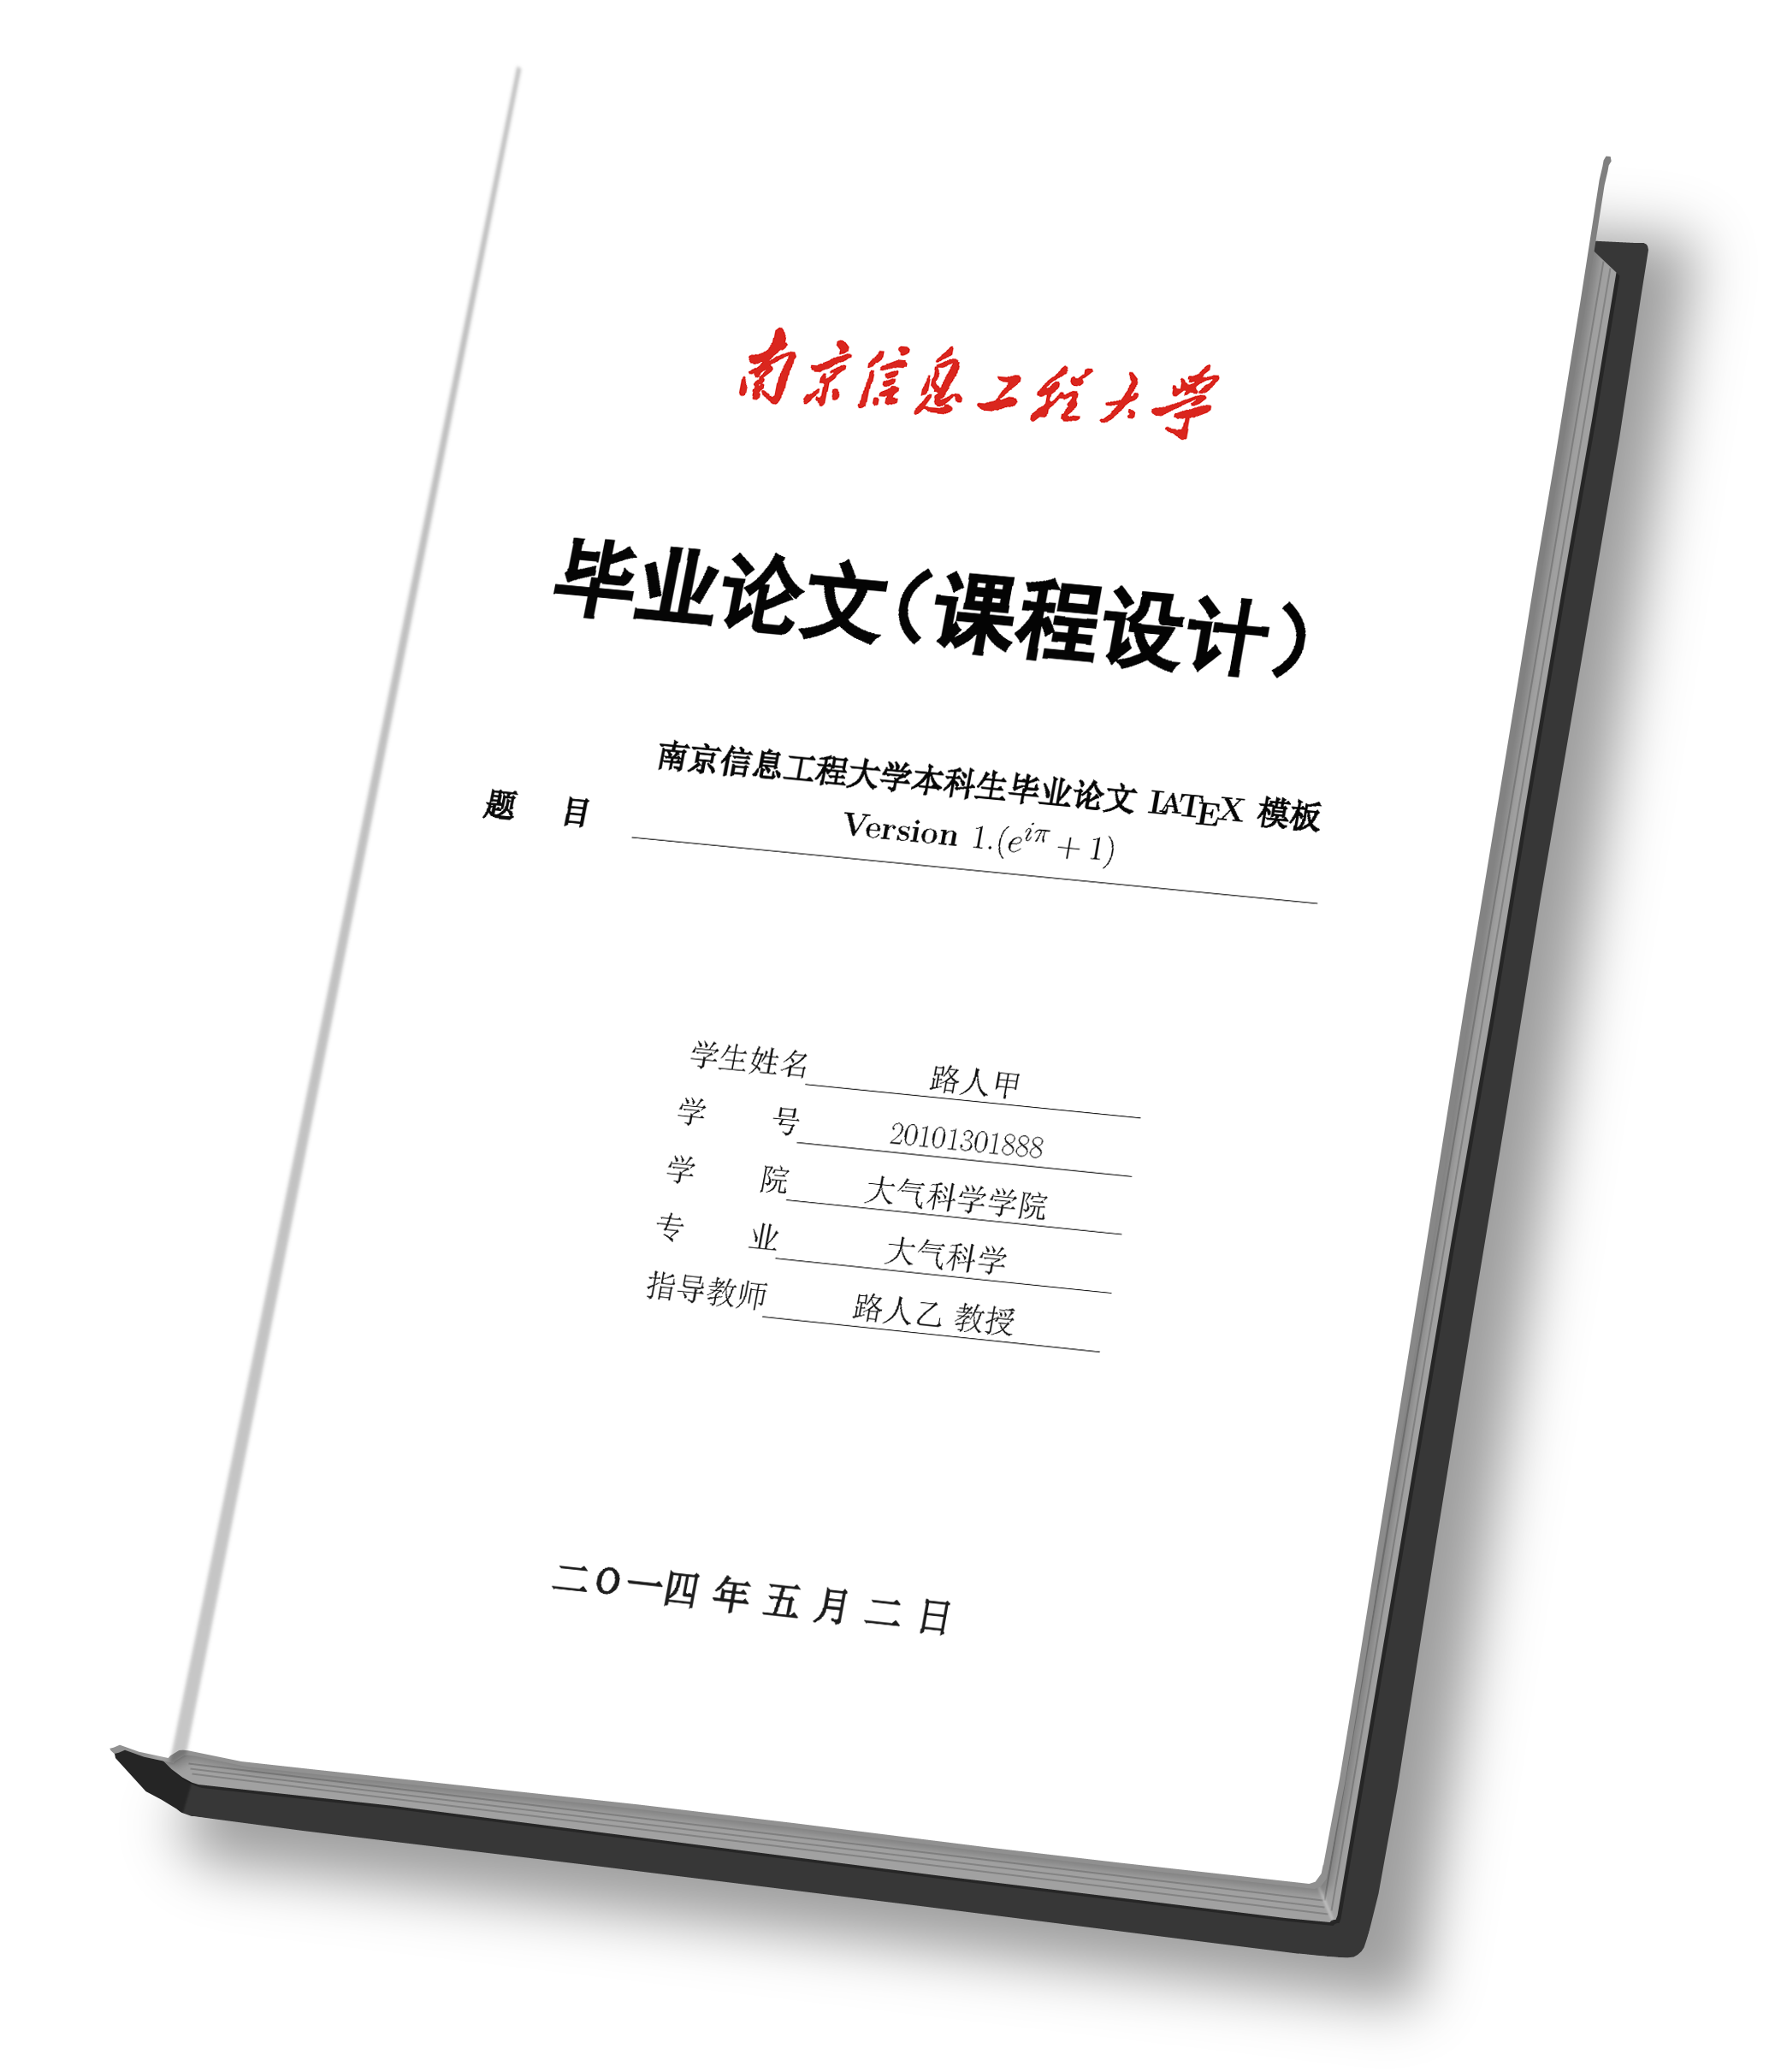
\includegraphics[width=0.6\textwidth]{figs/color/face.png}
\caption{南京信息工程大学本科生毕业论文\LaTeX 模板封面展示}
\label{nuist_face}
\end{figure}

图~\ref{nuist_face}~就是插入到文档中的图片,下面展示一下操作的代码:

{\color{green!50!black}
\begin{verbatim}
\begin{figure}[htbp!]
\centering
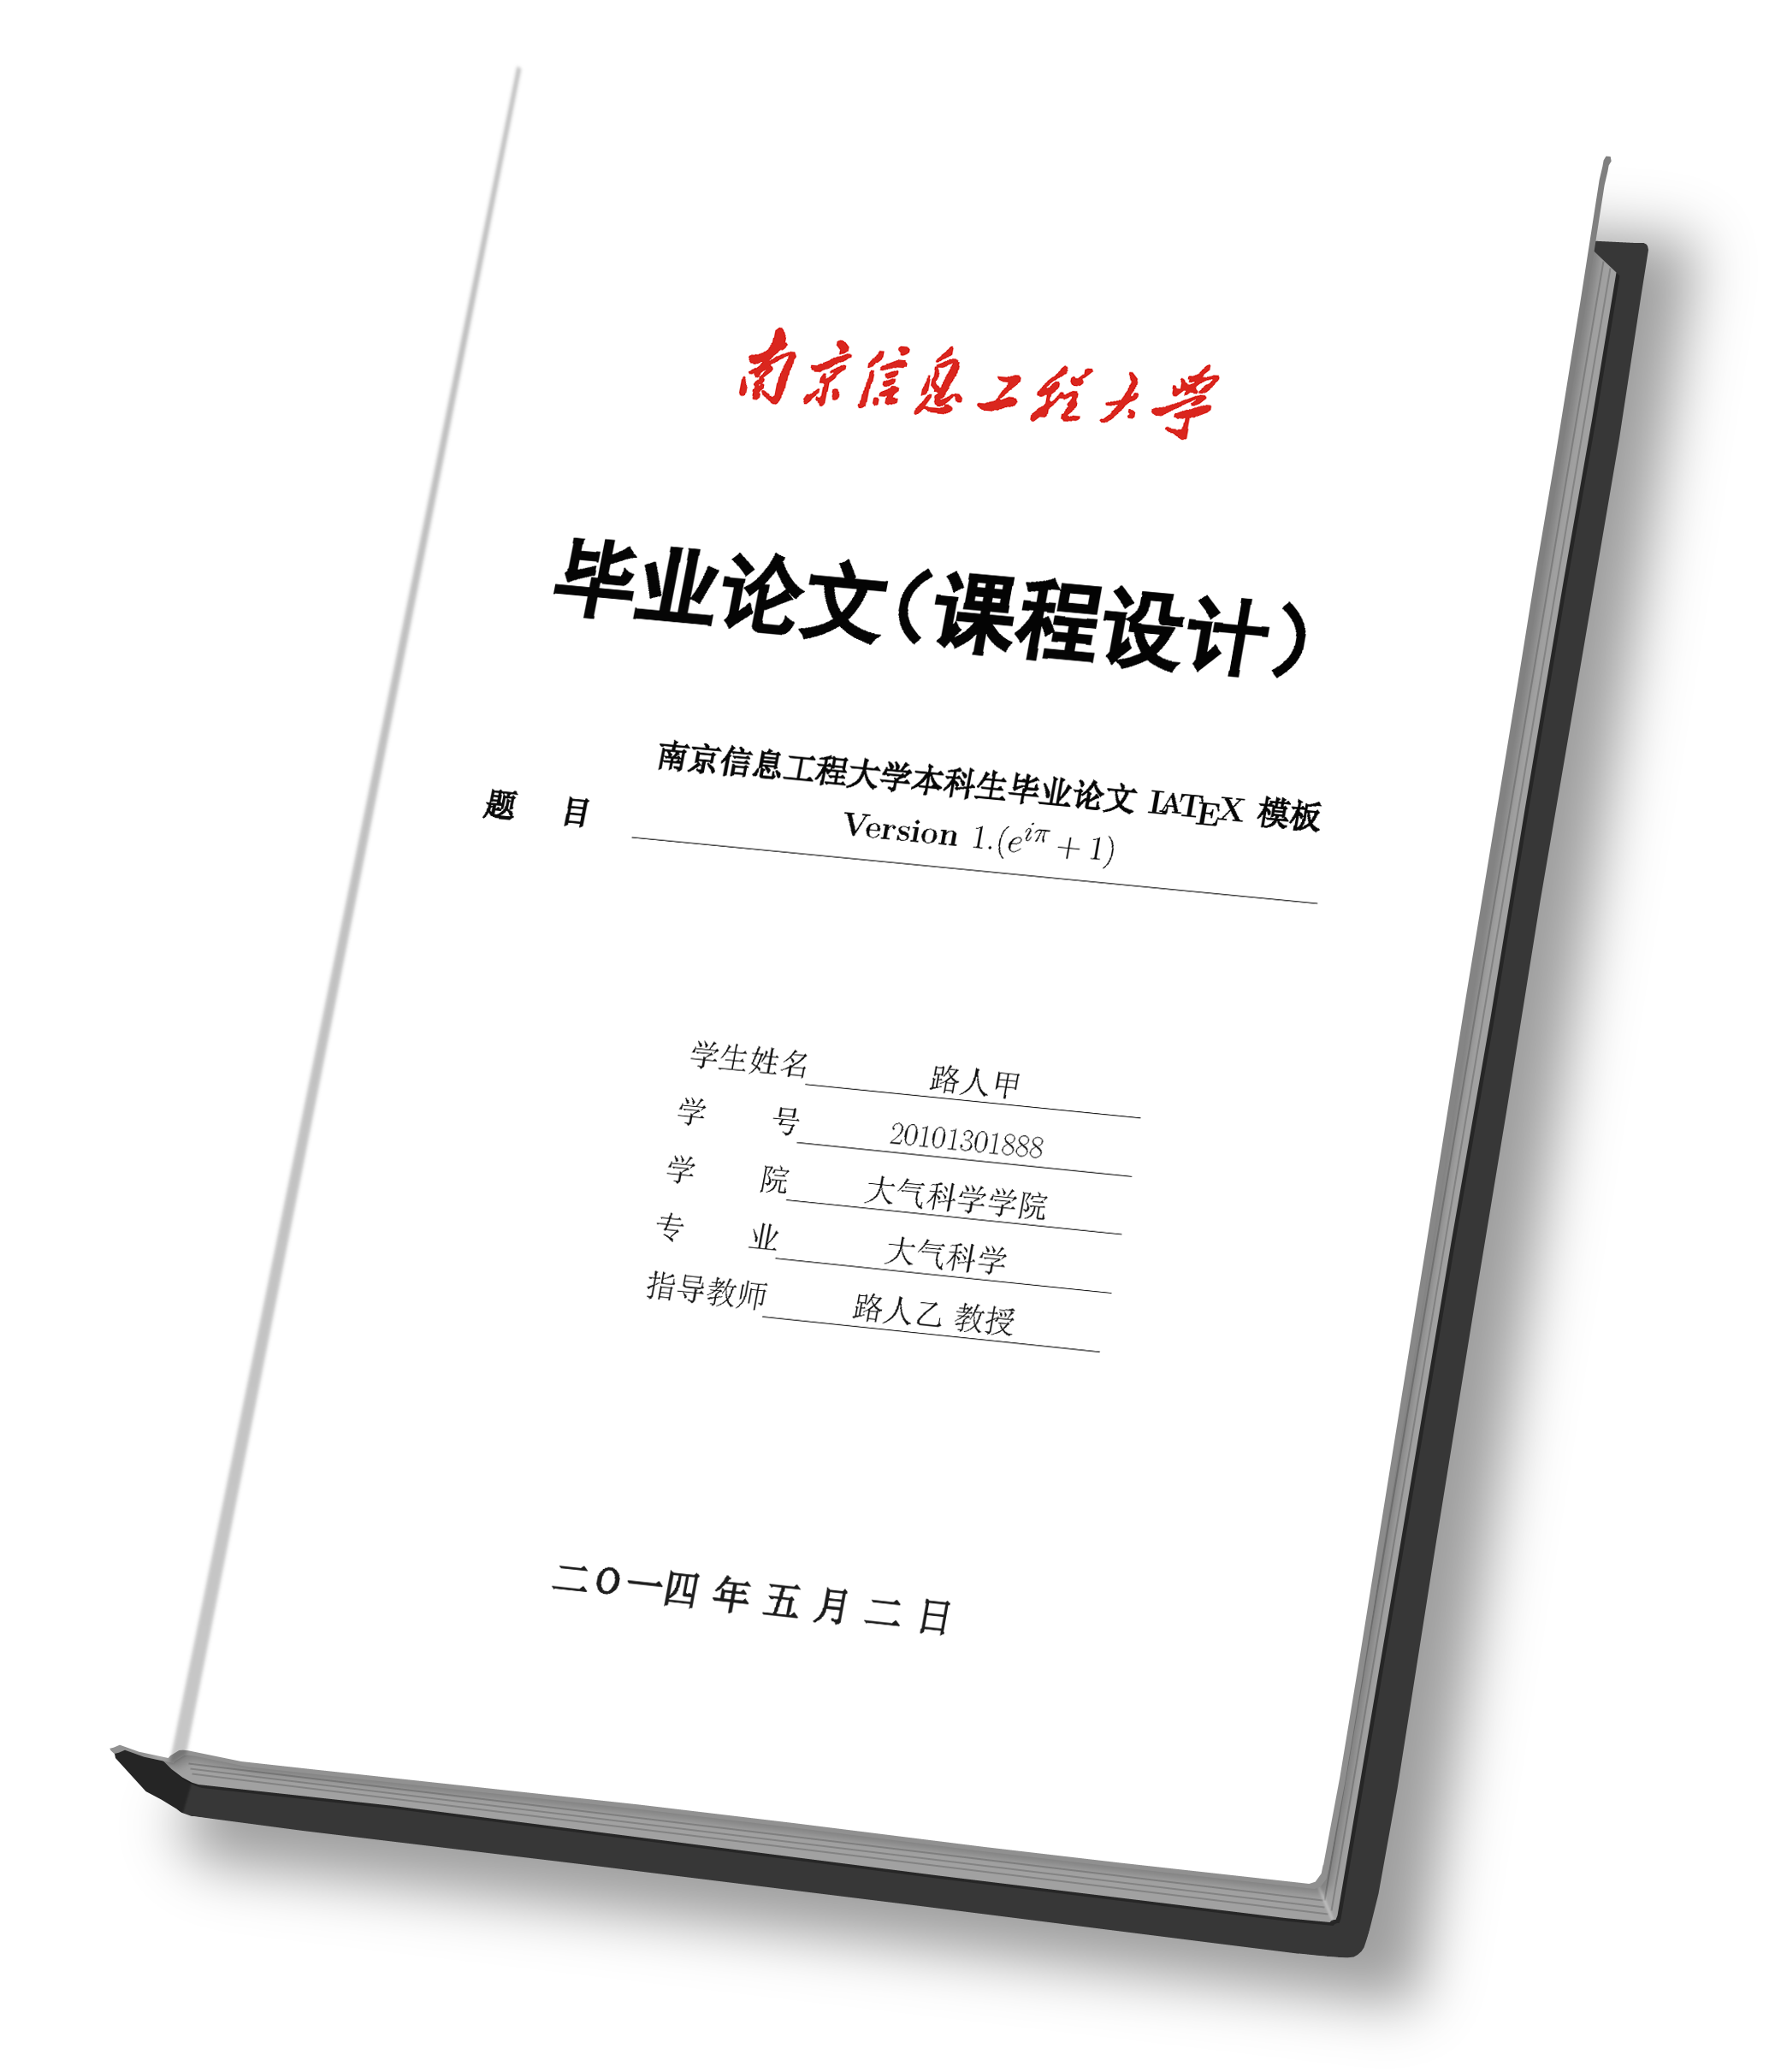
\includegraphics[width=0.6\textwidth]{figs/color/face.png}
\caption{南京信息工程大学本科生毕业论文\LaTeX 模板封面展示}
\label{nuist_face}
\end{figure}
\end{verbatim}
}
\subsection{并列图及添加子图标题}
大家在做论文时的时候经常需要两幅图并排的情况,还记得在word用鼠标一点点的拖动吗,通常拖到最后两幅图安排得还是不尽如人意,就算搞定了一组,下一组又要拖呀拉呀的。当然稍稍高明一点可以借助word的宏命令来控制,但word中宏的学习曲线十分的陡峭,大家在网上找到的宏,自己想重新定制一下,也是比较困难的。下面来看看\LaTeX 是怎样精确控制并排图片占位大小的,从而使其各占一半水平空间。如图~\ref{cn_map}~。

\begin{figure}[htbp!]
\centering
\includegraphics[width=0.5\textwidth]{figs/color/china1.png}\includegraphics[width=0.5\textwidth]{figs/color/china2.png}
\caption{中国地图展示(左图为素颜,右图为彩妆)}
\label{cn_map}
\end{figure}

其实现代码如下:
{\color{green!50!black}
\begin{verbatim}
\begin{figure}[htbp!]
\centering
\includegraphics[width=0.5\textwidth]{figs/color/china1.png}\includegraphics[width=0.5\textwidth]{figs/color/china2.png}
\caption{中国地图展示(左图为素颜,右图为彩妆)}
\label{cn_map}
\end{figure}
\end{verbatim}
}
是不是感觉图~\ref{cn_map}~的标题不太专业,也想给左右两个子图各加一个标题?那其实也很简单,只要引入subfigure宏包就可以实现。实现后效果如图~\ref{subfig_cn_map}~。

\begin{figure}[htbp!]
\centering
\subfigure[素颜\label{fig:sub1}]{\includegraphics[width=0.5\textwidth]{china1.png}}\subfigure[彩妆\label{fig:sub2}]{\includegraphics[width=0.5\textwidth]{china2.png}}
\caption{中国地图展示}
\label{subfig_cn_map}
\end{figure}

当然我们在引用的时候,可以引用母图,如图~\ref{subfig_cn_map}~,也可以引用子图,如图~\ref{fig:sub1}~,图~\ref{fig:sub2}~。好了让我们来看实现的代码吧。

{\color{green!50!black}
\begin{verbatim}

\begin{figure}[htbp!]
\centering
\subfigure[素颜\label{fig:sub1}]{\includegraphics[width=0.5\textwidth]{china1.png}}
\subfigure[彩妆\label{fig:sub2}]{\includegraphics[width=0.5\textwidth]{china2.png}}
\caption{中国地图展示}
\label{subfig_cn_map}
\end{figure}
\end{verbatim}
}

最后再给出一个例子,例如大家在做EOF分析时,可能要两个模态之间进行对比,我们知道每一个模态场都有一个时间序列与其对应,所以这样我们还可能用到$2\times 2$形式的图片排列方式,这时我们可以用下面的命令来实现:结果如图~\ref{fig:eof_12}~。

{\color{green!50!black}
\begin{verbatim}
\begin{figure}[htbp]

\center
\subfigure[第一模态]{\label{eof_1}
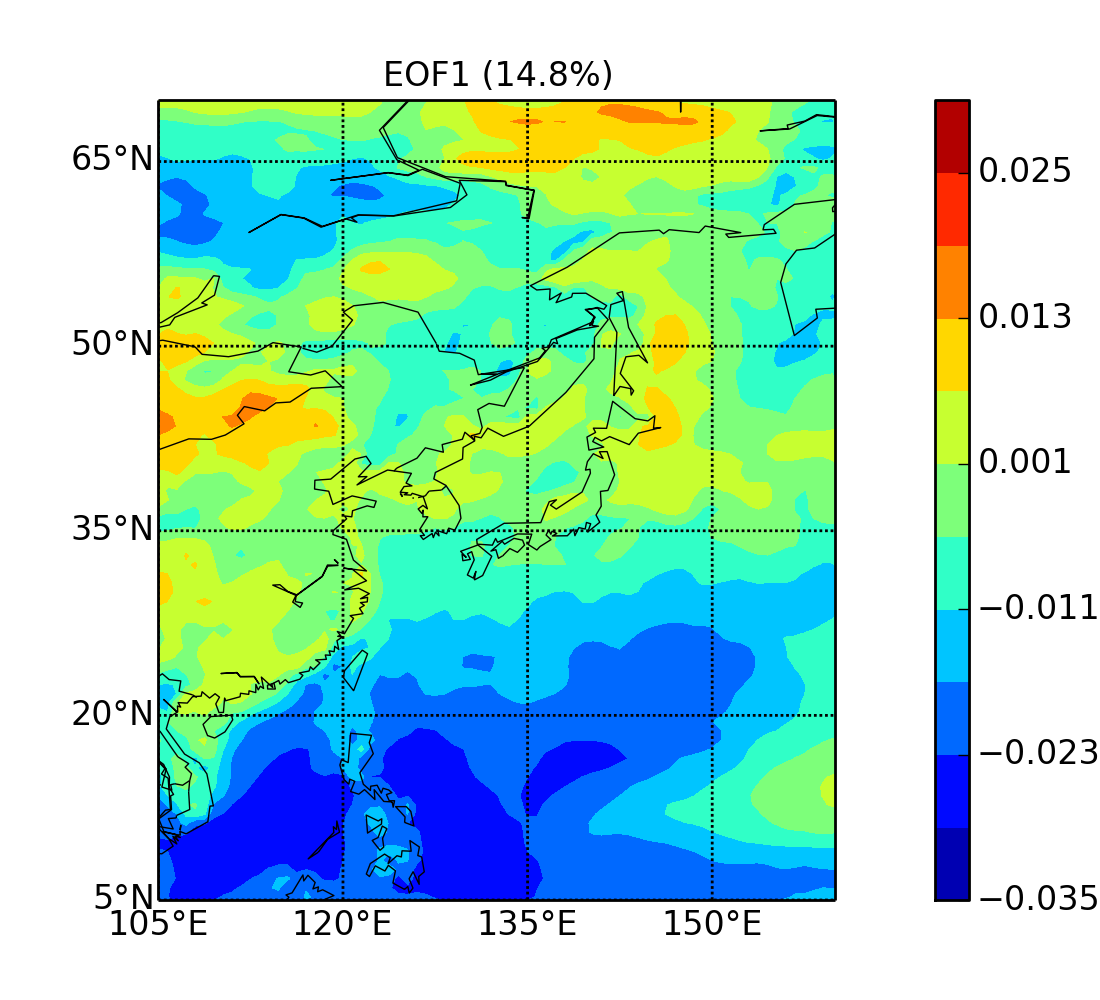
\includegraphics[width=0.5\textwidth]{eof1.png}
}\subfigure[第二模态]{\label{eof_2}
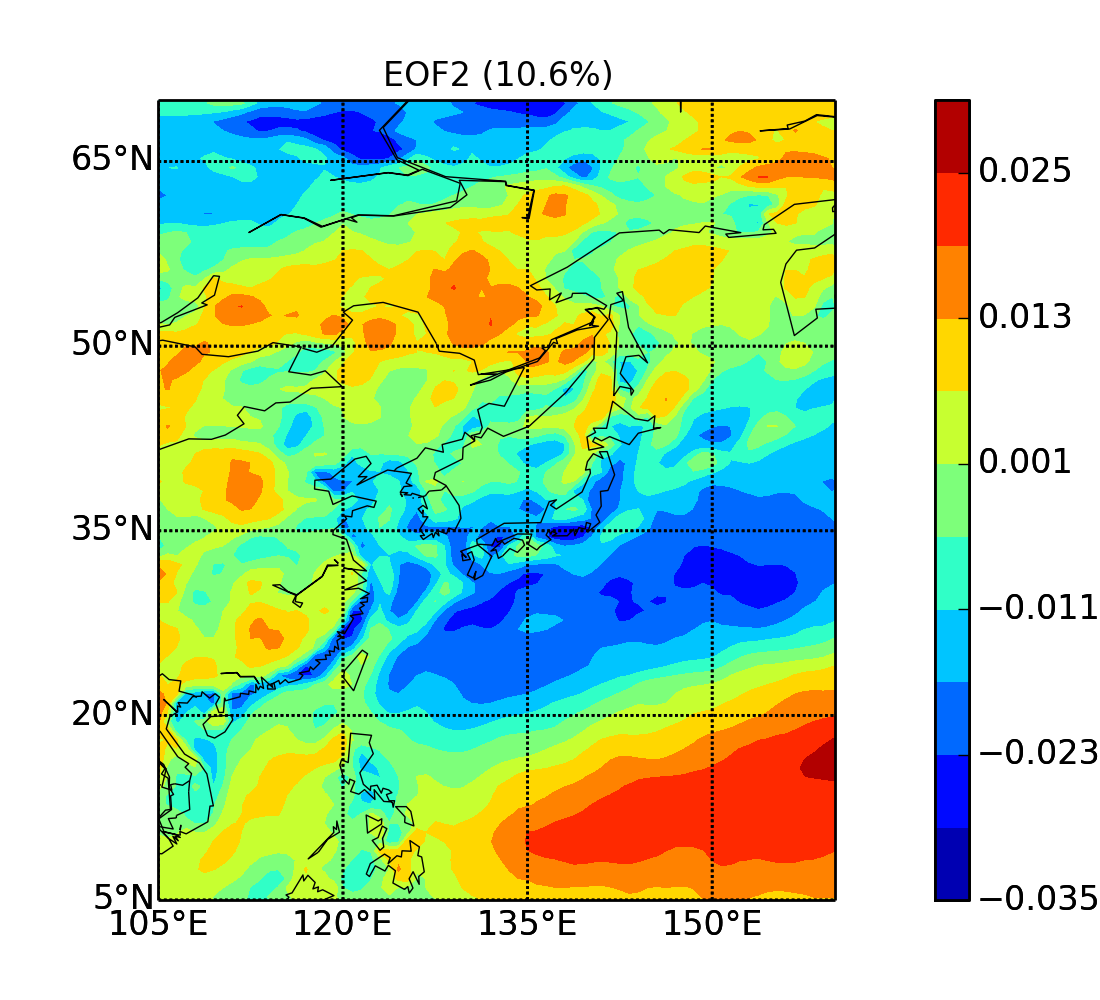
\includegraphics[width=0.5\textwidth]{eof2.png}
}
\\
\subfigure[第一模态对应的时间系数]{\label{eof_t1}
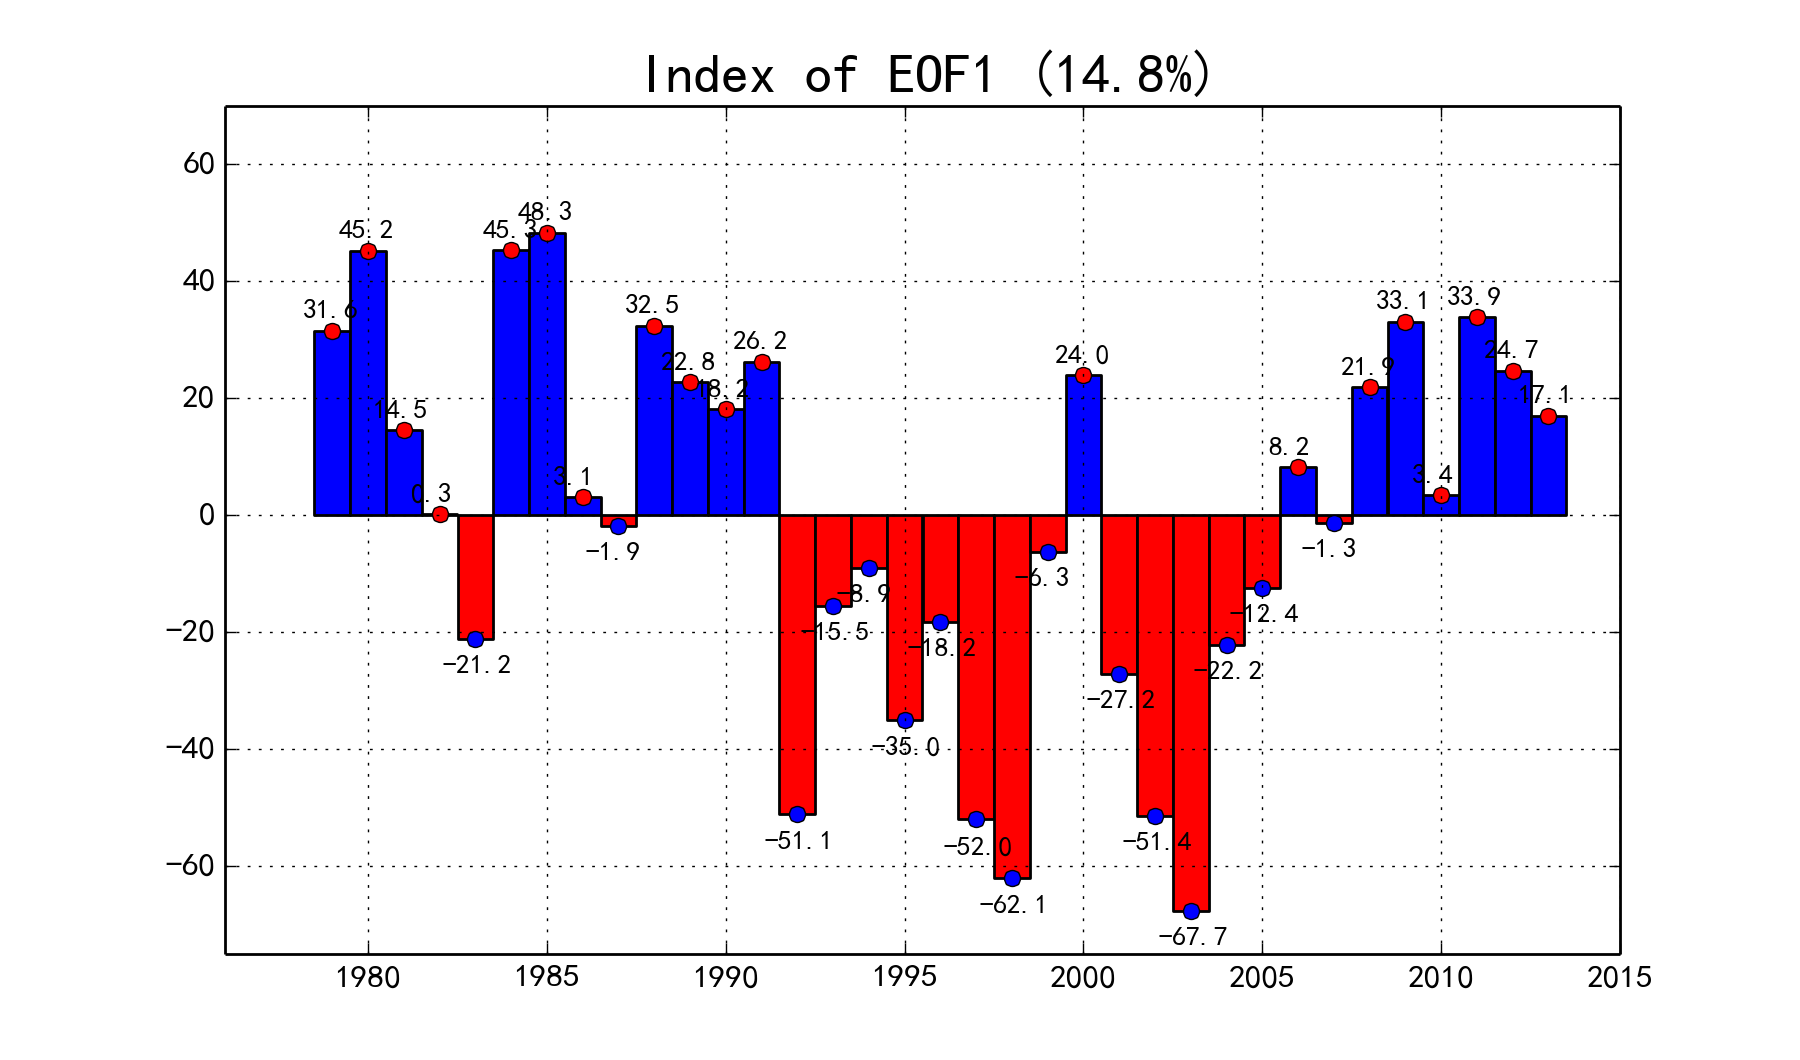
\includegraphics[width=0.5\textwidth]{t1.png}
}\subfigure[第二模态对应的时间系数]{\label{eof_t2}
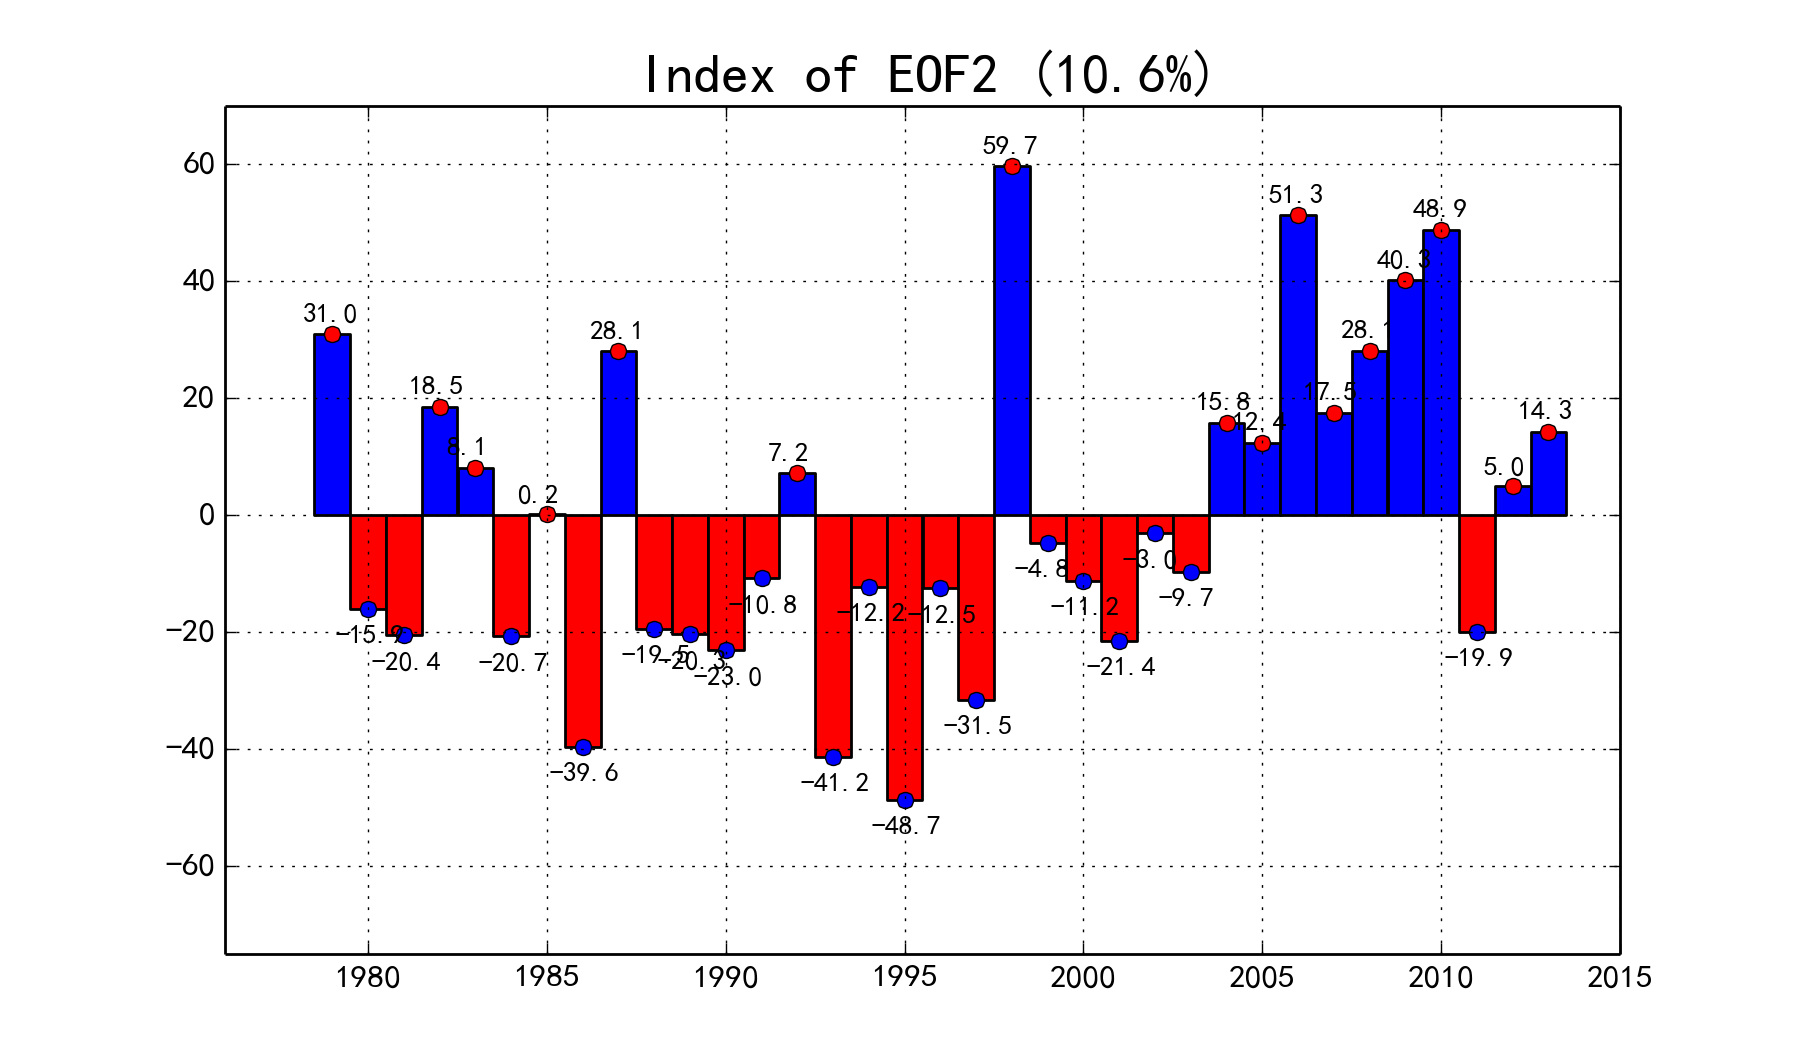
\includegraphics[width=0.5\textwidth]{t2.png}
}
\caption{ABLH的EOF分析结果(第一第二模态及其时间系数)}\label{fig:eof_12}
\end{figure}
\end{verbatim}
}


\begin{figure}[htbp]

\center
\subfigure[第一模态]{\label{eof_1}
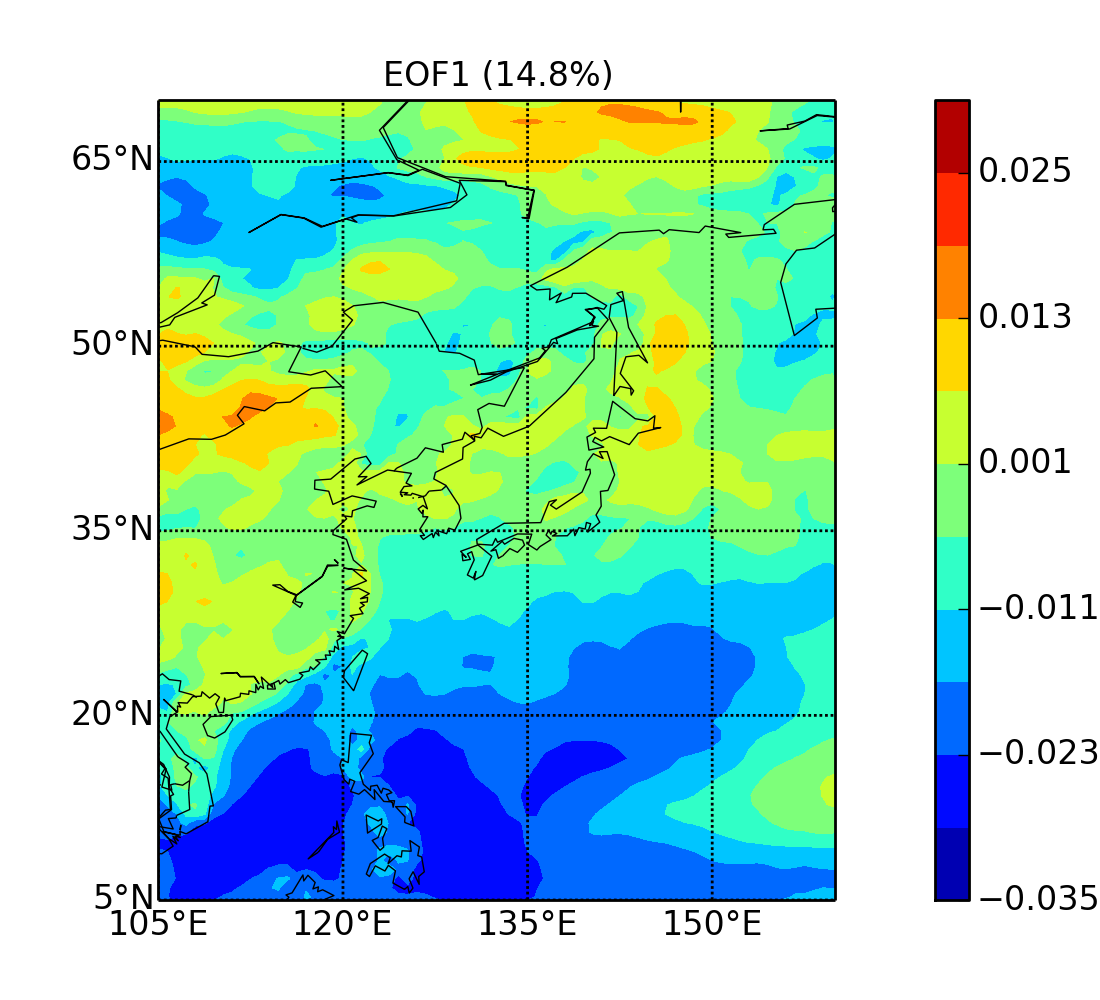
\includegraphics[width=0.5\textwidth]{eof1.png}
}\subfigure[第二模态]{\label{eof_2}
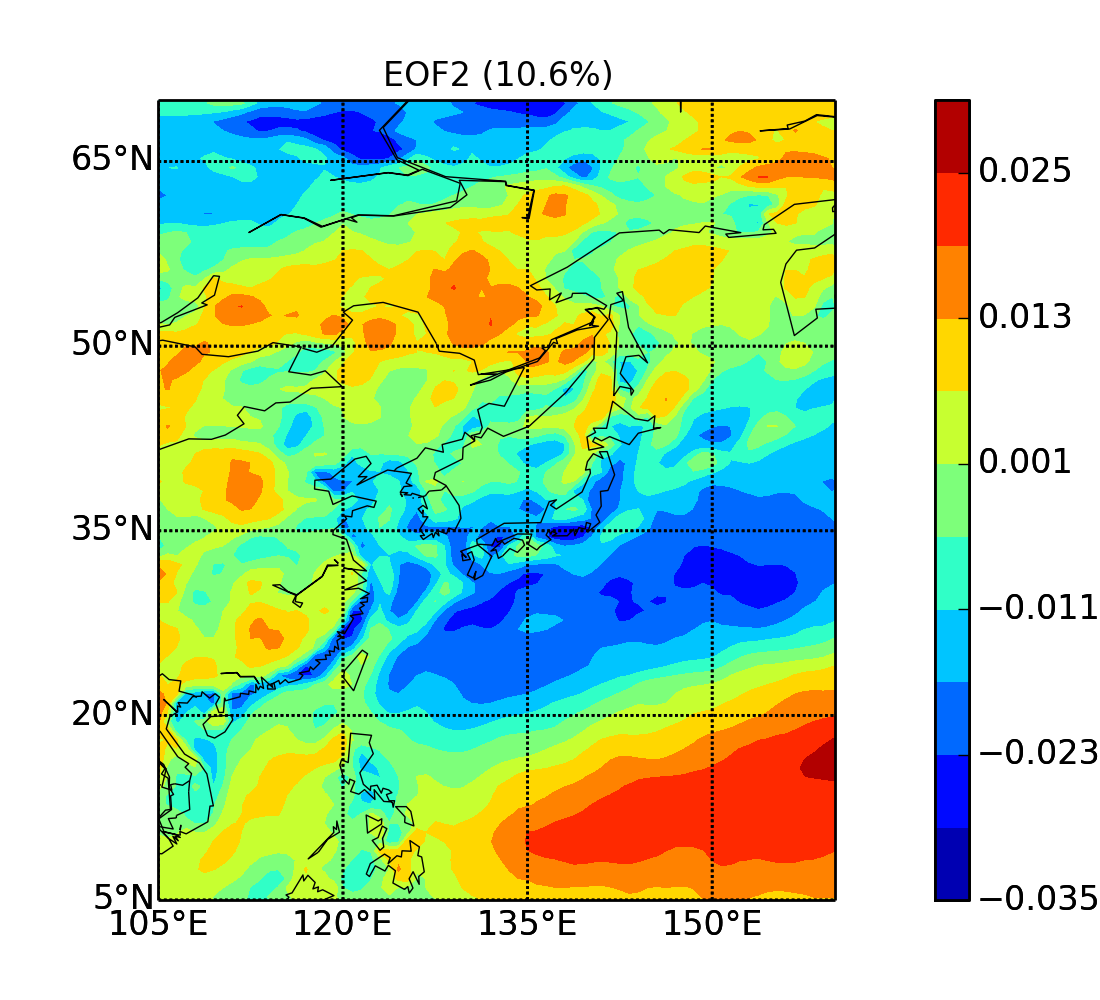
\includegraphics[width=0.5\textwidth]{eof2.png}
}
\\
\subfigure[第一模态对应的时间系数]{\label{eof_t1}
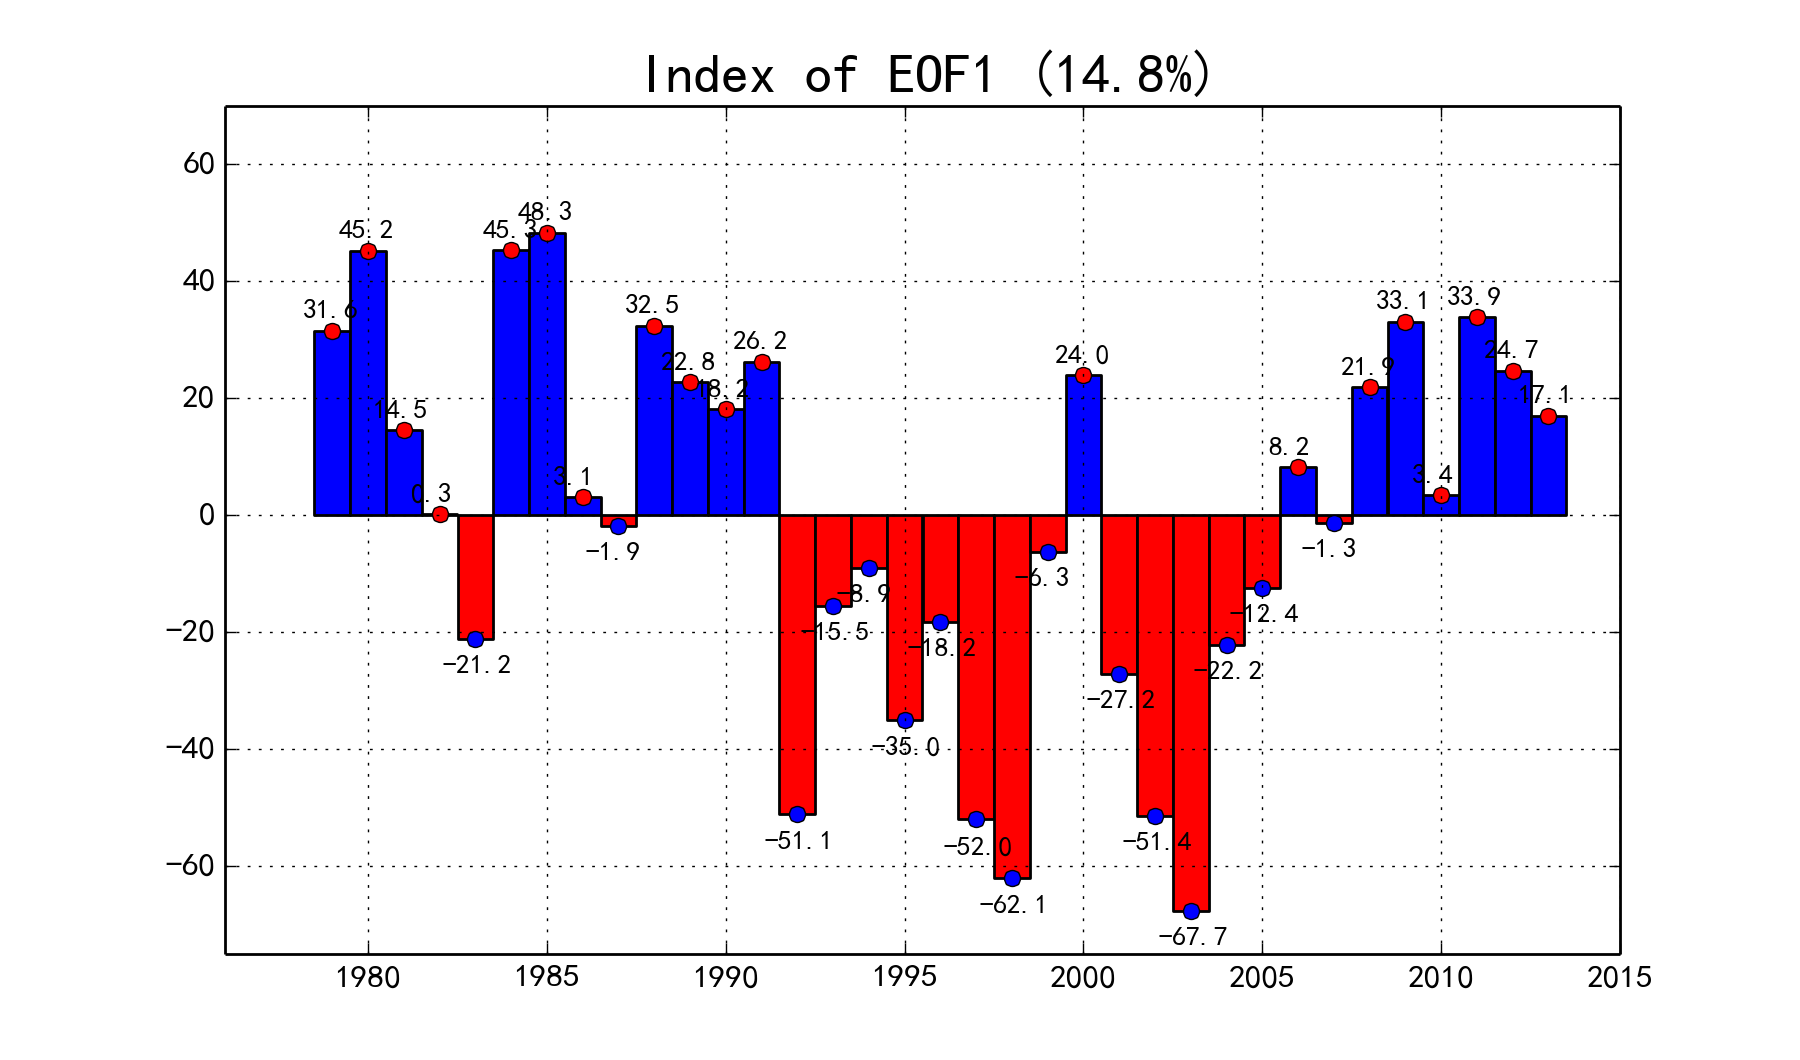
\includegraphics[width=0.5\textwidth]{t1.png}
}\subfigure[第二模态对应的时间系数]{\label{eof_t2}
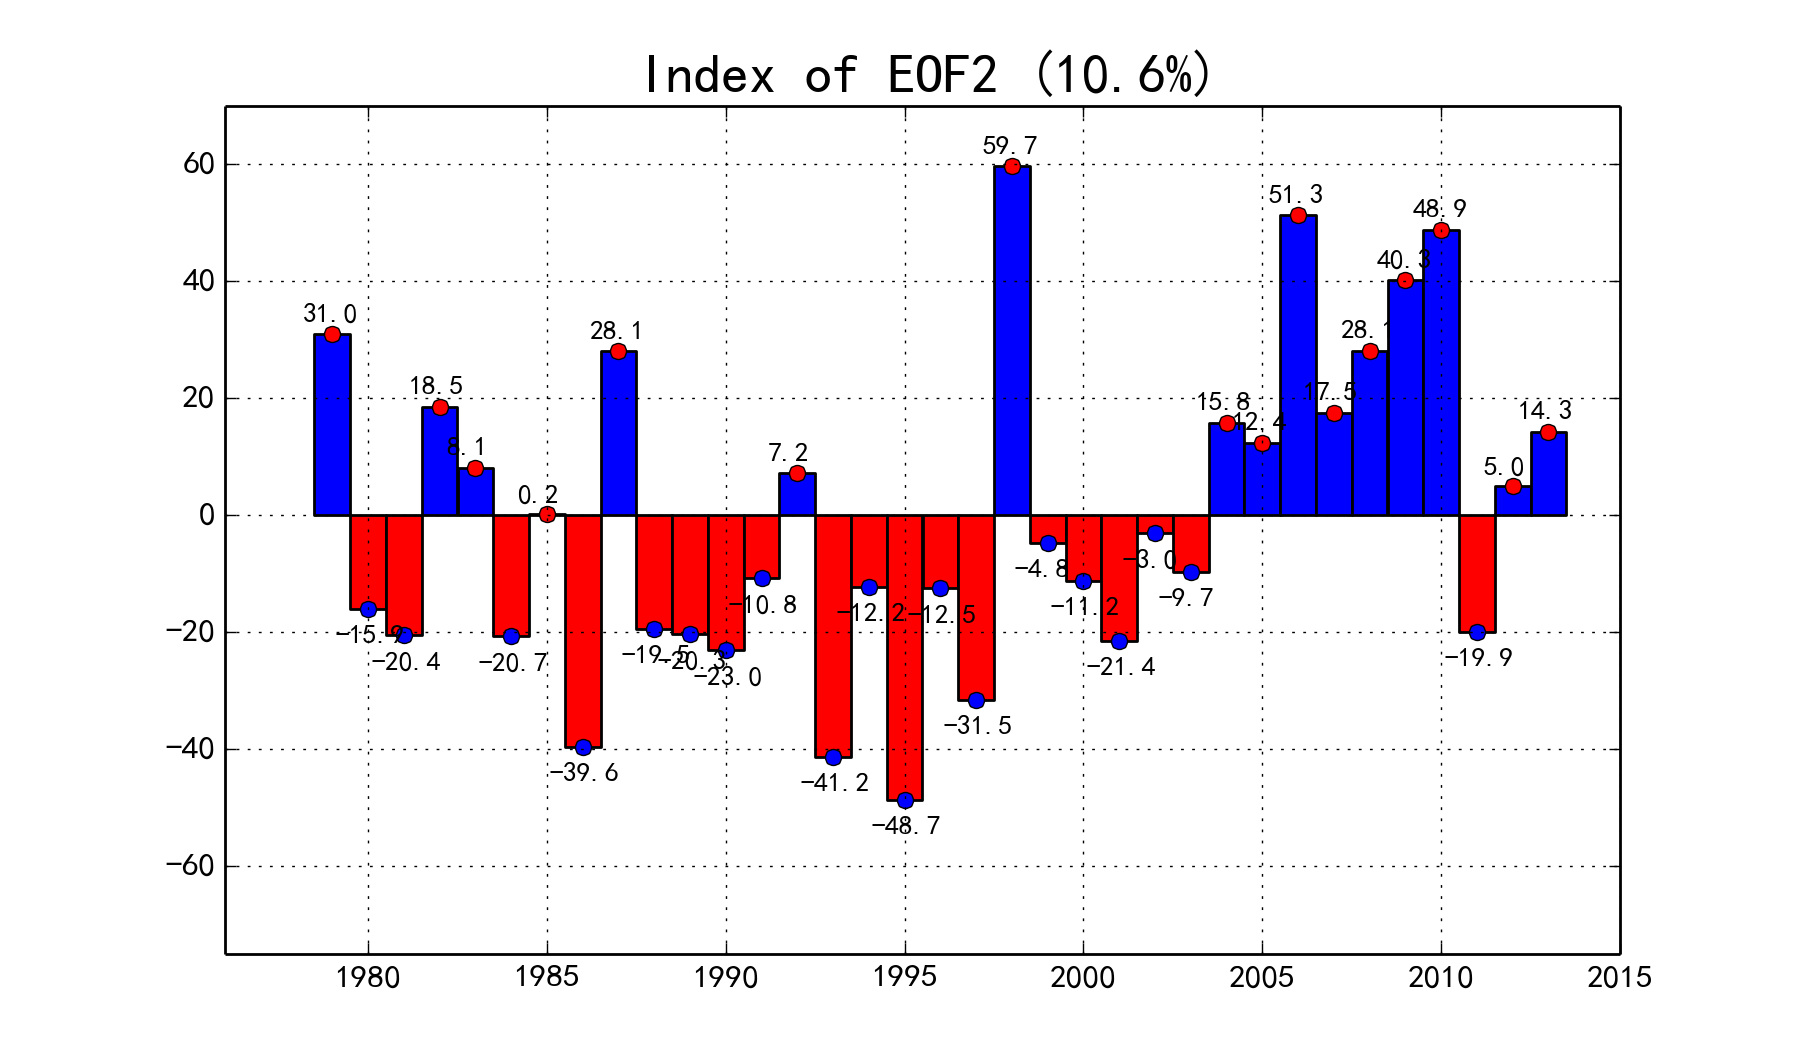
\includegraphics[width=0.5\textwidth]{t2.png}
}
\caption{ABLH的EOF分析结果(第一第二模态及其时间系数)}\label{fig:eof_12}
\end{figure}
朋友们应该也发现奥秘所在了,对,就是那个双斜线$ \backslash\backslash$的作用,双斜线在\LaTeX 排版系统中就是换行的命令,知道了这一点,大家可以随意安排自己的图片了,可以用$2\times 3$或者$3\times 2$来摆放自己插图了。


\subsection{图片文件夹的指定}
细心的朋友可能会发现生成~\ref{subfig_cn_map}~和图~\ref{cn_map}~所用的代码在指定图片路径时的写法不同,一种是全路径,另一种是只有图片名称。这是为什么呢?原因很简单。为了在写作时引用图片方便,本文在导言区写上这样的\verb|\graphicspath{{figs/color/}}|一名命令,来宏观地指定图片所存放的位置。

这一功能的好处就是,对于有的同学电子文档和打印文档所用图片色彩格式不同,这样只要一条命令就可以切换到另一个文件夹了,比较实用。
\subsection{图序号动态更新}

用word时,还有一种情况就是当我们突然想在文章中间补加一幅图时,后面图的编号及段落中对图的引用都要手工来改动,这是一件十分令人烦躁的事情,但\LaTeX 可以做到自动调整。

\section{排版表格}
\LaTeX 中生成简单的表格还是比较方便的,可以用tabular 环境来实现。下面就来做一个论文中经常用到的三线表,如表~\ref{table_1}~。

\begin{table}[htbp!]

\caption{本模板中所用的宏包及功能}\label{table_1}

\begin{tabular}{ccccccccc}
\whline 
宏包名称 & amsmath&caption2&geometry&ulem&xcolor&setspace&hyperref&titletoc \\ 
\hline 
作用 & 数学公式&定制标题&页面设置&下划线&颜色&行距&超链接&目录样式 \\ 
\whline 
\end{tabular}
\end{table}

其实现代码如下:
{\color{green!50!black}
\begin{verbatim}
\begin{table}[htbp!]
\caption{本模板中所用的宏包及功能}\label{table_1}
\begin{tabular}{ccccccccc}
\whline 
宏包名称 & amsmath&caption2&geometry&ulem&xcolor&setspace&hyperref&titletoc \\ 
\hline 
作用 & 数学公式&定制标题&页面设置&下划线&颜色&行距&超链接&目录样式 \\ 
\whline 
\end{tabular}
\end{table}
\end{verbatim}
}
如果表格比较长,那就要用到跨页表格排版宏包longtable了。基本的表格排版情况就介绍这么多,大家感兴趣自己慢慢去探索吧。
\section{排版参考文献及引用}
本模板采用thebibliography环境来排版参考文献,对如下代码进行编译即可得到本文后面的参考文献摆放形式。
{\color{green!50!black}
\begin{verbatim}
\begin{thebibliography}{99}\setlength{\itemsep}{-0.1mm}
\begin{spacing}{1.2}
\zihao{-5}
\bibitem{x1}The Not So Short Introduction to 
\LaTeX2e \ by Tobias Oetiker, Hubert Partl, Irene Hyna and Elisabeth Schlegl.
\bibitem{x0}李平.\LaTeX2e 及常用宏包使用指南[M].清华大学出版社,2004.
\bibitem{x3}罗振东,葛向阳.排版软件\LaTeX 简明手册[M].第二版.北京:电子工业出版社,2003.
\end{spacing}
\end{thebibliography}
\end{verbatim}
}
引用文献条目时使用\verb|\ucite{}|命令,例如代码\verb|\ucite{x1}|和\verb|\ucite{x2}|就可以产生\ucite{x1}和\ucite{x2}上标。


\section{写在后面}
时间过得真快,从五一动手,到码字码到这里差不多快三天了。这么短的时间,不管模板本身还是说明文档肯定还是不够完善的。但时间所迫,也必须到这了。

有人也许行会产生疑问,word不是用着挺好的吗,干嘛要学这个,干嘛要用这个写论文呢?其实要我回答呢,的确是这样的,随便用哪个排版软件用顺手了就好了,没人强迫你做什么,关键在于自己是怎么想。

去年笔者在写学年论文时,就“吃了亏”,先是用\LaTeX 写的,生成的pdf格式的文档,但是最后学院不认,说必须用word版的,无奈后来又用word重排了一遍。(所以这里插一句,如果真有哪位朋友想用这个模板,请“严重”地考虑这个“严重”的后果,弄不好到最后,只能用它排个打印版玩玩,电子版还得word 去。)

而对笔者来说,无所谓,不是天空经常会飘来五个字儿,叫“这都不是事儿”嘛,人生本就是向死之生,要是总走直线,太快到终点了怎么办?所以人生的要义就在于走“弯路”,走得越“弯”走得越长嘛。

\section{第二版!新鲜出炉!}
两年以后,这个模板又被重新更新了一次(原作者应该并没有更新过(因为并不能联系到原作者(sigh。因为每年的格式都会进行一些修改,所以按照现在的格式改了一下模板,特别是字号和字体,并且针对一些问题进行了修改(以下如果感觉麻烦可以略过233),不过要注意的是,NUIST一向不欢迎PDF格式的论文提交,因此此模板,正如原作者说的那样,需要慎用、慎用和慎用。\par
对于无法复制PDF的问题,由于CTeX的设置问题解决方案比较复杂,本模板采用修改字体为Adobe Song Std 的方法,不过如果要完整解决此问题请参考\url{https://www.zhihu.com/question/32207411}这个回答,不过低版本的CTeX+WinEdit套装中CTeX版本过低无法使用,可以考虑升级全部宏包(此方法可能会导致WinEdit宏包冲突,慎用)也可以等新版本的套装(听说快出了)。\par
关于行距的问题,虽然word和LaTeX的行距计算方法相同(行距:一行文字的基线(Base Line)到下一行文字的基线的距离,详见\cite{x4}),但是修改出的文章行距感觉比word略宽,不知道为什么,期待后人能解决此问题!\par
\section{修订者的话}
说完了专业问题,聊点其他的话题好了。笔者接触LaTeX也蛮久了,从数学建模就用自己修改的模板进行论文写作,到写毕业论文时还是用LaTeX,感觉长文章基本脱离Word了,不是不会用(不自夸地说,论Word排版本人也完全可以完成长文章的各种排版工作),而是感觉Word排出来的东西一点也不美。\par
Knuth感觉自己写的东西被编辑排成了渣,于是很不开心地花时间做了个排版系统;乔布斯觉得手机太丑,于是自己做了个iPhone。我也有这种感觉,且不说Word那蛋疼的贪心断行算法(最常见的例子的是加上了数学公式和英文字符后完全不对齐的右边界)、令人抓狂的图片摆放,就拿最简单的来说,一个写作软件,为什么要让用户找不到如何更新引用!我知道那复杂的域代码和目录生成,然而一个一个设置它们的格式实在令人发指,并且一个不小心,版面就跑到十万八千里以外。不过什么是美呢?想来对我来说的话就是“Simple is the best”,能让电脑自动计算的事情完全不应该由手工来做,能动脑解决的就绝不动手。\par
世界是因为懒人才变得舒适,但“懒”往往需要的是Critical Thinking和Curiosity,而对我来说,对美这一形而上的终极目标的追求促使我探索这个世界,而对这个世界无穷无尽的美好的好奇让我在探索的过程中不太无聊。\par
引用百度百科(好吧我最唾弃百度的各种玩意了)TeX的词条的一句话吧:
\begin{quote}
  TeX是一种乐趣: 使用TeX不仅仅是一种工作手段,也是一种乐趣。它有挑战,也有荣誉。很多人在熟悉了TeX之后都开始把使用TeX作为一种爱好,而不是一件枯燥无味的劳动。
\end{quote}
我使用TeX就是因为它简洁明快,让我专注于内容而不需要纠结于无聊的排版疏忽,随意调节结构而不用担心随之而来的格式更新,总而言之就是这个样子\footnote{面白い}。\par
\addcontentsline{toc}{section}{参考文献}
\begin{thebibliography}{99}\setlength{\itemsep}{-0.1mm}
\begin{spacing}{1.2}
\zihao{-5}

\bibitem{x1}The Not So Short Introduction to \LaTeX2e \ by Tobias Oetiker, Hubert Partl, Irene Hyna and Elisabeth Schlegl.

\bibitem{x2}李平.\LaTeX2e 及常用宏包使用指南[M].北京:清华大学出版社,2004.

\bibitem{x3}罗振东,葛向阳.排版软件\LaTeX 简明手册[M].第二版.北京:电子工业出版社,2003.
\bibitem{x4}刘海洋. \LaTeX 入门[M]
\end{spacing}
\end{thebibliography}



\thanking
感谢春风之骀荡,感谢细雨之无声,感谢花枝之袅娜,感谢土地之坚忍。
\vspace{5em}
{\color{red}
\heartpar{鉴于您已经读到这里,噢,也可能是用鼠标拖到这里的,但这不是什么大不了的区别,重要的是您手指或者眼睛一定有一些疲倦了吧? 这段文字能与您相遇,笔者心里已经满是感激,为了表达这样的心情,特奉上红心一颗,望看官笑纳! -- Lee贰零壹肆年伍月叁日于南京}

}
\end{document}





